\newpage
\section{نمودار و مشخصات موارد کاربردساختاردهی‌شده}

\subsection{زیرسیستم کاربری}

\vspace{2cm}
\begin{center}
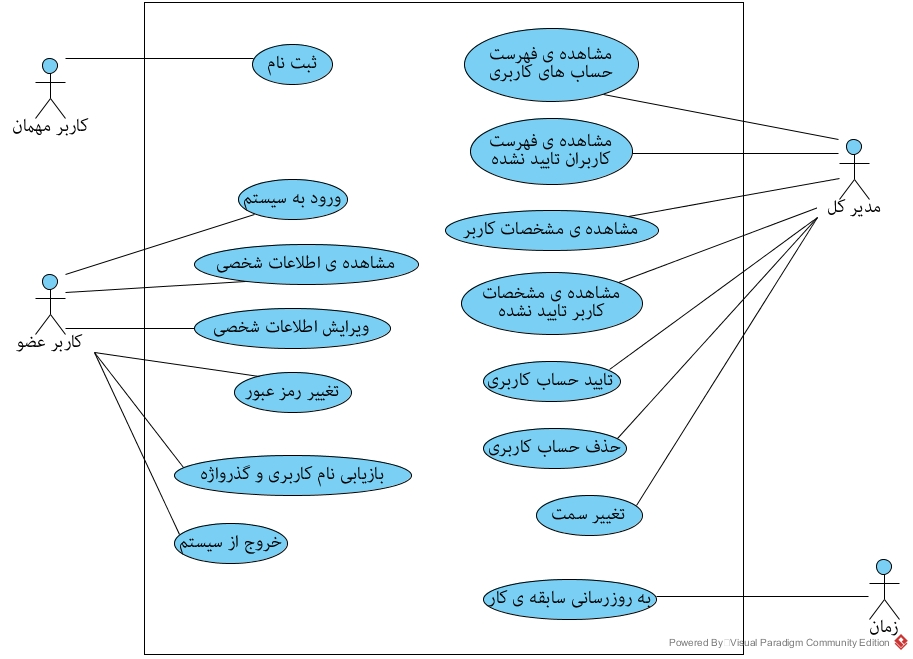
\includegraphics[width=\textwidth]{Diagrams/Accounting.jpg}
\end{center}

\newpage


\begin{tabular}{|p{2cm}|p{10cm}|}
\hline
نام
&
ثبت نام
\\
\hline
شناسه
&
1
\\
\hline
توصیف کوتاه
&
کاربر مهمان در سامانه یک حساب کاربری ایجاد می کند.
\\
\hline
اکتور اولیه
&
کاربر مهمان
\\
\hline
اکتور ثانویه
&

\\
\hline
شرایط ابتدایی
&

\\
\hline
سناریوی اصلی
&
1-	کاربر مهمان با انتخاب گزینه ثبت نام این مورد کاربرد را شروع می کند.
\newline
2-	کاربر مشخصات خود شامل نام، نام خانوادگی، کد ملی ، شماره تلفن، تاریخ تولد، مدرک تحصیلی ، وضعیت تاهل ، سابقه کار و... را وارد میکند.
\newline
3-	با انتخاب گزینه ثبت اطلاعات، مشخصات کاربر مهمان برای مدیر ارسال می شود.
\\
\hline
شرایط نهایی
&
سیستم اطلاعات حساب کاربری را برای مدیر ارسال می کند.
\\
\hline
سناریوی جایگزین
&

\\
\hline
\end{tabular}

\vspace{2cm}


\begin{tabular}{|p{2cm}|p{10cm}|}
\hline
نام
&
مشاهده فهرست حساب های کاربری
\\
\hline
شناسه
&
2
\\
\hline
توصیف کوتاه
&
مدیر فهرست حسابهای کاربری را مشاهد می کند.
\\
\hline
اکتور اولیه
&
مدیرکل
\\
\hline
اکتور ثانویه
&

\\
\hline
شرایط ابتدایی
&
مدیر در سیستم وارد شده باشد.
\\
\hline
سناریوی اصلی
&
1-	مدیر با انتخاب گزینه فهرست حسابهای کاربری، این مورد کاربرد را شروع می کند.
\newline
2-	سیستم حسابهای کاربری موجود را به ترتیب زمان ایجاد نمایش می دهد.
\\
\hline
شرایط نهایی
&
فهرست حسابهای کاربری نمایش داده می شود.
\\
\hline
سناریوی جایگزین
&

\\
\hline
\end{tabular}

\vspace{2cm}


\begin{tabular}{|p{2cm}|p{10cm}|}
\hline
نام
&
مشاهده فهرست کاربران تایید نشده
\\
\hline
شناسه
&
3
\\
\hline
توصیف کوتاه
&
مدیر فهرست حسابهای کاربران مهمان را مشاهد می کند.
\\
\hline
اکتور اولیه
&
مدیرکل
\\
\hline
اکتور ثانویه
&

\\
\hline
شرایط ابتدایی
&
مدیر در سیستم وارد شده باشد.
\\
\hline
سناریوی اصلی
&
1-	مدیر با انتخاب گزینه فهرست کاربران مهمان، این مورد کاربرد را شروع می کند.
\newline
2-	سیستم حسابهای کاربران مهمان موجود را به ترتیب زمان ایجاد نمایش می دهد.
\\
\hline
شرایط نهایی
&
فهرست کاربران مهمان نمایش داده می شود.
\\
\hline
سناریوی جایگزین
&

\\
\hline
\end{tabular}

\vspace{2cm}


\begin{tabular}{|p{2cm}|p{10cm}|}
\hline
نام
&
مشاهده مشخصات کاربر
\\
\hline
شناسه
&
4
\\
\hline
توصیف کوتاه
&
مدیر مشخصات کاربر را مشاهده می کند.
\\
\hline
اکتور اولیه
&
مدیرکل
\\
\hline
اکتور ثانویه
&

\\
\hline
شرایط ابتدایی
&
مدیر در سیستم وارد شده باشد.
\\
\hline
سناریوی اصلی
&
1-	مدیرکل با انتخاب کاربر از فهرست کاربران، این مورد کاربرد را شروع می کند.
\newline
2-	سیستم مشخصات کاربر را نمایش می دهد.
\\
\hline
شرایط نهایی
&
مشخصات کاربر نمایش داده می شود.
\\
\hline
سناریوی جایگزین
&

\\
\hline
\end{tabular}

\vspace{2cm}

\begin{tabular}{|p{2cm}|p{10cm}|}
\hline
نام
&
مشاهده مشخصات کاربر تاییدنشده
\\
\hline
شناسه
&
5
\\
\hline
توصیف کوتاه
&
مدیر مشخصات کاربر مهمان را مشاهده می کند.
\\
\hline
اکتور اولیه
&
مدیرکل
\\
\hline
اکتور ثانویه
&

\\
\hline
شرایط ابتدایی
&
مدیر در سیستم وارد شده باشد.
\\
\hline
سناریوی اصلی
&
1-	مدیرکل با انتخاب کاربر مهمان از فهرست کاربران مهمان، این مورد کاربرد را شروع می کند.
\newline
2-	سیستم مشخصات کاربر مهمان را نمایش می دهد.
\\
\hline
شرایط نهایی
&
مشخصات مهمان کاربر نمایش داده می شود.
\\
\hline
سناریوی جایگزین
&

\\
\hline
\end{tabular}

\vspace{2cm}

\begin{tabular}{|p{2cm}|p{10cm}|}
\hline
نام
&
تایید حساب کاربری
\\
\hline
شناسه
&
6
\\
\hline
توصیف کوتاه
&
مدیر کاربر مهمان را به عنوان یک عضو تایید می کند.
\\
\hline
اکتور اولیه
&
مدیرکل
\\
\hline
اکتور ثانویه
&

\\
\hline
شرایط ابتدایی
&
مدیر در سیستم وارد شده باشد.
\\
\hline
سناریوی اصلی
&
1-	مدیرکل با انتخاب گزینه تایید مهمان، این مورد کاربرد را شروع می کند.
\newline
2-	سیستم مشخصه عضویت کاربر را از مهمان به عضو تغییر می دهد.
\\
\hline
شرایط نهایی
&
مشخصه عضویت کاربر از مهمان به عضو تغییر کند.
\\
\hline
سناریوی جایگزین
&

\\
\hline
\end{tabular}

\vspace{2cm}


\begin{tabular}{|p{2cm}|p{10cm}|}
\hline
نام
&
حذف حساب کاربری
\\
\hline
شناسه
&
7
\\
\hline
توصیف کوتاه
&
مدیر حساب کاربری را از سیستم حذف می کند.
\\
\hline
اکتور اولیه
&
مدیر کل
\\
\hline
اکتور ثانویه
&

\\
\hline
شرایط ابتدایی
&
مدیر در سیستم وارد شده باشد.
\\
\hline
سناریوی اصلی
&
1-	مدیرکل با انتخاب گزینه حذف، این مورد کاربرد را شروع می کند.
\newline
2-	سیستم حساب کاربری را حذف می کند.
\\
\hline
شرایط نهایی
&
حذف حساب کاربری از سیستم
\\
\hline
سناریوی جایگزین
&

\\
\hline
\end{tabular}

\vspace{2cm}


\begin{tabular}{|p{2cm}|p{10cm}|}
\hline
نام
&
تغییر سمت
\\
\hline
شناسه
&
8
\\
\hline
توصیف کوتاه
&
مدیر سمت کاربر عضو را تغییر می دهد.
\\
\hline
اکتور اولیه
&
مدیر کل
\\
\hline
اکتور ثانویه
&

\\
\hline
شرایط ابتدایی
&
مدیر در سیستم وارد شده باشد.
\\
\hline
سناریوی اصلی
&
1-	مدیر با انتخاب یک سمت برای کاربر عضو، این مورد کاربرد را شروع می کند.
\newline
2-	سیستم سمت انتخاب شده را برای کاربر عضو ثبت می کند.
\\
\hline
شرایط نهایی
&
سمت کاربر عضو تغییر کند.
\\
\hline
سناریوی جایگزین
&

\\
\hline
\end{tabular}

\vspace{2cm}


\begin{tabular}{|p{2cm}|p{10cm}|}
\hline
نام
&
به روز رسانی سابقه‌کار
\\
\hline
شناسه
&
9
\\
\hline
توصیف کوتاه
&
پس از گذشت زمان معین، سابقه کار کاربر عضو به روز می شود.
\\
\hline
اکتور اولیه
&
مدیر کل
\\
\hline
اکتور ثانویه
&

\\
\hline
شرایط ابتدایی
&

\\
\hline
سناریوی اصلی
&
1-	پس از گذشت هر 6 ماه از زمان ساخت حساب کاربری، این مورد کاربرد شروع می شود.
\newline
2-	سیستم اطلاعات مربوط به سابقه کار را به علاوه ی 0.5 می کند.
\\
\hline
شرایط نهایی
&
اطلاعات مربوط به سابقه کار به علاوه 0.5 شود.
\\
\hline
سناریوی جایگزین
&

\\
\hline
\end{tabular}

\vspace{2cm}

\begin{tabular}{|p{2cm}|p{10cm}|}
\hline
نام
&
ورود به سیستم
\\
\hline
شناسه
&
10
\\
\hline
توصیف کوتاه
&
کاربر با وارد کردن نام و کلمه عبور وارد سیستم می شود.
\\
\hline
اکتور اولیه
&
کاربر عضو
\\
\hline
اکتور ثانویه
&

\\
\hline
شرایط ابتدایی
&

\\
\hline
سناریوی اصلی
&
1- کاربر با این انتخاب گزینه ورود به سیستم این مورد کاربرد را شروع می کند
\newline
2- کاربر نام کاربری و رمز عبور خود را وارد می کند.
\newline
3- با انتخاب گزینه ورود، کاربر اقدام به ورود می کند.
\newline
4- سیستم اطلاعات کاربر را بررسی می کند.
\newline
5- اگر نام کاربری و رمز عبور کاربر مطابقت داشتند:
\newline
5.1- کاربر وارد سیستم می شود.
\newline
در غیر اینصورت:
\newline
5.2- پیغام خطا جهت ورود صحیح اطلاعات داده می شود.
\\
\hline
شرایط نهایی
&
ورود کاربر و یا مشاهده پیغام خطا
\\
\hline
سناریوی جایگزین
&

\\
\hline
\end{tabular}

\vspace{2cm}


\begin{tabular}{|p{2cm}|p{10cm}|}
\hline
نام
&
ویرایش اطلاعات شخصی
\\
\hline
شناسه
&
11
\\
\hline
توصیف کوتاه
&
کاربر می تواند اطلاعات شخصی خود را تغییر دهد.
\\
\hline
اکتور اولیه
&
کاربر عضو
\\
\hline
اکتور ثانویه
&

\\
\hline
شرایط ابتدایی
&
کاربر به سیستم وارد شده باشد.
\\
\hline
سناریوی اصلی
&
1- کاربر با انتخاب گزینه ویرایش اطلاعات، مورد کاربرد را شروع می کند.
\newline
2- کاربر یک یا چند مورد از اطلاعات شخصی از جمله: نام، نام خانوادگی، کد ملی، شماره تلفن، تاریخ تولد، مدرک تحصیلی، وضعیت تاهل، سابقه کار و ... را تغییر می دهد.
\newline
3- با انتخاب گزینه ثبت اطلاعات، سیستم مشخصات تغییر کرده کاربر را ثبت می کند. 
\\
\hline
شرایط نهایی
&
ثبت مشخصات تغییر کرده کاربر
\\
\hline
سناریوی جایگزین
&

\\
\hline
\end{tabular}

\vspace{2cm}

\begin{tabular}{|p{2cm}|p{10cm}|}
\hline
نام
&
تغییر رمز عبور
\\
\hline
شناسه
&
12
\\
\hline
توصیف کوتاه
&
کاربر رمز عبور خود در سیستم را تغییر می دهد.
\\
\hline
اکتور اولیه
&
کاربر عضو
\\
\hline
اکتور ثانویه
&

\\
\hline
شرایط ابتدایی
&
کاربر به سیستم وارد شده باشد.
\\
\hline
سناریوی اصلی
&
1- کاربر عضو با انتخاب گزینه تغییر رمز عبور این مورد کاربرد را اجرا می کند.
\newline
2- کاربر رمز عبور قبل و رمز عبور جدید را وارد می کند.
\newline
3- با انتخاب گزینه تایید، کاربر عملیات تغییر رمز عبور را آغاز می کند.
\newline
4- اگر رمز عبور قبل با رمز عبور کاربر یکسان بود:
\newline
4.1- سیستم رمز عبور جدید را جایگزین رمز عبور قبلی می کند.
\newline
در غیر اینصورت:
\newline
4.2- سیستم پیغام خطایی مبنی بر درست نبودن رمز عبور قبلی نمایش می دهد.
\\
\hline
شرایط نهایی
&
جایگزین شدن رمز عبور جدید با رمز عبور قبلی و یا نمایش پیغاغم خطا
\\
\hline
سناریوی جایگزین
&

\\
\hline
\end{tabular}

\vspace{2cm}

\begin{tabular}{|p{2cm}|p{10cm}|}
\hline
نام
&
بازیابی نام کاربری و کلمه عبور
\\
\hline
شناسه
&
13
\\
\hline
توصیف کوتاه
&
در صورتی که کاربر نام کاربری یا رمز عبور خود را فراموش کرده باشد،  می تواند با وارد کردن ایمیل آنها را بازیابی می کند.
\\
\hline
اکتور اولیه
&
کاربر عضو
\\
\hline
اکتور ثانویه
&

\\
\hline
شرایط ابتدایی
&
کاربر به سیستم وارد شده باشد.
\\
\hline
سناریوی اصلی
&
1- کاربر با انتخاب گزینه بازیابی اطلاعات، این مورد کاربرد را شروع می کند.
\newline
2- کاربر آدرس پست الکترونیکی خود را در سیستم وارد می کند.
\newline
3- با انتخاب گزینه بازیابی، کاربر موافقت خود را با ارسال ایمیل بازیابی اعلام می کند.
\newline
4- اگر ایمیل داده شده در سیستم موجود باشد:
\newline
4.1- سیستم پیامی حاوی نام کاربری و کلمه عبور را به ایمیل داده شده ارسال می کند.
\newline
در غیر اینصورت:
\newline
4.2- سیستم پیغام خطایی مبنی بر اشتباه بودن ایمیل وارد شده نمایش می دهد.
\\
\hline
شرایط نهایی
&
ارسال ایمیل حاوی نام کاربری و کلمه عبور و یا نمایش پیغام خطا
\\
\hline
سناریوی جایگزین
&

\\
\hline
\end{tabular}

\vspace{2cm}

\begin{tabular}{|p{2cm}|p{10cm}|}
\hline
نام
&
خروج از سیستم
\\
\hline
شناسه
&
14
\\
\hline
توصیف کوتاه
&
کاربر از سیستم خارج می شود.
\\
\hline
اکتور اولیه
&
کاربر عضو
\\
\hline
اکتور ثانویه
&

\\
\hline
شرایط ابتدایی
&
کاربر وارد سیستم شده باشد.
\\
\hline
سناریوی اصلی
&
1- کاربر با انتخاب گزینه خروج، این مورد کاربرد را شروع می کند.
\newline
2- سیستم کاربر را از سیستم خارج می کند.
\\
\hline
شرایط نهایی
&
خروج کاربر از سیستم
\\
\hline
سناریوی جایگزین
&

\\
\hline
\end{tabular}

\vspace{2cm}

\begin{tabular}{|p{2cm}|p{10cm}|}
\hline
نام
&
مشاهده اطلاعات شخصی
\\
\hline
شناسه
&
15
\\
\hline
توصیف کوتاه
&
کاربر اطلاعات شخصی خود را در سیستم مشاهده می کند.
\\
\hline
اکتور اولیه
&
کاربر عضو
\\
\hline
اکتور ثانویه
&

\\
\hline
شرایط ابتدایی
&
کاربر وارد سیستم شده باشد.
\\
\hline
سناریوی اصلی
&
1- کاربر با انتخاب گزینه ی مشاهده پروفایل، این مورد کاربرد را شروع میکند.
\newline
2- سیستم مشخصات کاربر شامل نام، نام خانوادگی، کد ملی ، شماره تلفن، تاریخ تولد، مدرک تحصیلی ، وضعیت تاهل ، سابقه کار و... را نمایش می دهد. 
\\
\hline
شرایط نهایی
&
نمایش مشخصات کاربر
\\
\hline
سناریوی جایگزین
&

\\
\hline
\end{tabular}


\newpage
\subsection{زیرسیستم تولید و نگهداری}

\vspace{2cm}
\begin{center}
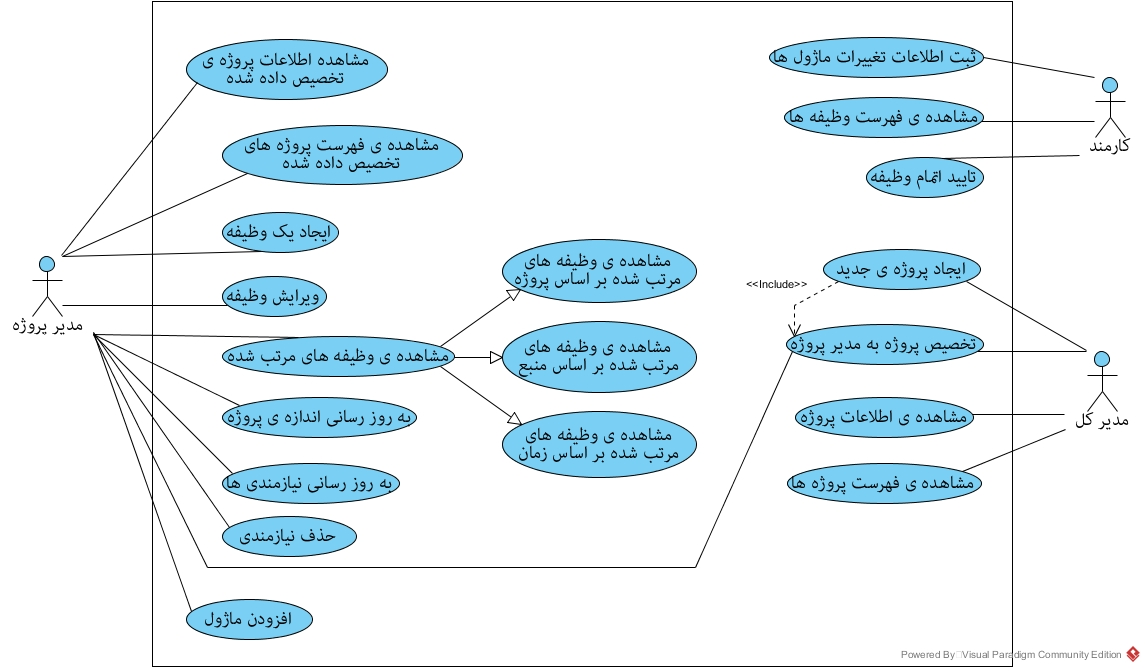
\includegraphics[width=\textwidth]{Diagrams/Development.jpg}
\end{center}

\newpage

\begin{tabular}{|p{2cm}|p{10cm}|}
\hline
نام
&
مشاهده  لیست پروژه های تخصیص داده شده
\\
\hline
شناسه
&
16
\\
\hline
توصیف کوتاه
&
لیستی از پروژه های تخصیص داده شده به یک مدیر پروژه، نمایش داده می شود.
\\
\hline
اکتور اولیه
&
مدیر پروژه
\\
\hline
اکتور ثانویه
&

\\
\hline
شرایط ابتدایی
&
مدیر پروژه وارد حساب کاربری خود شده باشد. 
\\
\hline
سناریوی اصلی
&
1-مدیر پروژه ، با انتخاب مشاهده  لیست پروژه های تخصیص داده شده  این مورد کاربرد را شروع می کند.
\newline
2-سیستم لیست پروژه های تخصیص داده شده به مدیر پروژه را نمایش می دهد
\\
\hline
شرایط نهایی
&
لیست پروژه های تخصیص داده شده به مدیر پروژه نمایش داده می شوند.
\\
\hline
سناریوی جایگزین
&

\\
\hline
\end{tabular}

\vspace{2cm}

\begin{tabular}{|p{2cm}|p{10cm}|}
\hline
نام
&
مشاهده اطلاعات پروژه تخصیص داده شده
\\
\hline
شناسه
&
17
\\
\hline
توصیف کوتاه
&
اطلاعات یک پروژه  تخصیص داده شده به مدیر پروژه نمایش داده می شود.
\\
\hline
اکتور اولیه
&
مدیر پروژه
\\
\hline
اکتور ثانویه
&

\\
\hline
شرایط ابتدایی
&
مدیر پروژه وارد حساب کاربری خود شده باشد
\\
\hline
سناریوی اصلی
&
1-مدیر پروژه ، با انتخاب مشاهده اطلاعات پروژه  تخصیص داده شده این مورد کاربرد را شروع می کند.
\newline
2-سیستم اطلاعات پروژه ی تخصیص داده شده انتخاب شده  توسط مدیر پروژه را نمایش می دهد

\\
\hline
شرایط نهایی
&
مدیر پروژه، اطلاعات پروژه ی تخصیص داده شده انتخاب شده  خود را مشاهده میکند.
\\
\hline
سناریوی جایگزین
&

\\
\hline
\end{tabular}

\vspace{2cm}

\begin{tabular}{|p{2cm}|p{10cm}|}
\hline
نام
&
ایجاد یک وظیفه
\\
\hline
شناسه
&
18
\\
\hline
توصیف کوتاه
&
مدیر پروژه براساس نیازمندی ها، یک وظیفه آماده تخصیص به کارمندان ایجاد میکند.
\\
\hline
اکتور اولیه
&
مدیر پروژه
\\
\hline
اکتور ثانویه
&

\\
\hline
شرایط ابتدایی
&
مدیر پروژه وارد حساب کاربری خود شده باشد. 
\\
\hline
سناریوی اصلی
&
1-مدیر پروژه ، با انتخاب ایجاد یک وظیفه  این مورد کاربرد را شروع می کند.
\newline
2- مدیر پروژه مشخصات وظیفه شامل : عنوان، زمان مورد نیاز و زمان پایان ، ماژول های درگیر و توضیحات لازم را وارد می کند. 
\newline
3-با انتخاب گزینه تایید توسط مدیر پروژه ، وظیفه ایجاد می شود.
\\
\hline
شرایط نهایی
&
ایجاد یک وظیفه
\\
\hline
سناریوی جایگزین
&

\\
\hline
\end{tabular}

\vspace{2cm}

\begin{tabular}{|p{2cm}|p{10cm}|}
\hline
نام
&
ویرایش وظیفه
\\
\hline
شناسه
&
19
\\
\hline
توصیف کوتاه
&
مدیر پروژه اطلاعات یک وظیفه ایجاد شده را ویرایش می کند. 
\\
\hline
اکتور اولیه
&
مدیر پروژه
\\
\hline
اکتور ثانویه
&

\\
\hline
شرایط ابتدایی
&
مدیر پروژه وارد حساب کاربری خود شده باشد. 
\\
\hline
سناریوی اصلی
&
1-مدیر پروژه ، با انتخاب ویرایش وظیفه  این مورد کاربرد را شروع می کند.
\newline
2- مدیر پروژه یک یا چند مورد از مشخصات وظیفه شامل : زمان مورد نیاز و زمان پایان ،وضعیت اتمام،کارمندان انجام دهنده،  ماژول های درگیر و توضیحات لازم را ویراش می کند. 
\newline
3-با انتخاب گزینه تایید توسط مدیر پروژه ، تغییرات دخیره می شوند.
\\
\hline
شرایط نهایی
&
تغییرات وظیفه دخیره می شوند.
\\
\hline
سناریوی جایگزین
&

\\
\hline
\end{tabular}

\vspace{2cm}

\begin{tabular}{|p{2cm}|p{10cm}|}
\hline
نام
&
مشاهده وظیفه های مرتب شده
\\
\hline
شناسه
&
20
\\
\hline
توصیف کوتاه
&
لیست مرتب شده وظیفه ها بر اساس معیار مورد نظر مدیر پروژه ، نمایش داده می شود.
\\
\hline
اکتور اولیه
&
مدیر پروژه
\\
\hline
اکتور ثانویه
&

\\
\hline
شرایط ابتدایی
&
مدیر پروژه وارد حساب کاربری خود شده باشد. 
\\
\hline
سناریوی اصلی
&
1-مدیر پروژه ، با انتخاب مشاهده وظیفه های مرتب شده، این مورد کاربرد را شروع می کند.
\newline
2- مدیر پروژه معیار مورد نظر خود برای مرتب سازی وظیفه ها را انتخاب می کند. 
\newline
3-سیستم لیست مرتب شده وظیفه ها را به مدیر پروژه نمایش می دهد.
\\
\hline
شرایط نهایی
&
لیست مرتب شده وظیفه ها به مدیر پروژه نمایش داده می شود.
\\
\hline
سناریوی جایگزین
&

\\
\hline
\end{tabular}

\vspace{2cm}

\begin{tabular}{|p{2cm}|p{10cm}|}
\hline
نام
&
مشاهده وظیفه های مرتب شده بر اساس پروژه
\\
\hline
شناسه
&
21
\\
\hline
شناسه پدر
&
20
\\
\hline
توصیف کوتاه  
&
لیست مرتب شده وظیفه ها بر اساس پروژه، نمایش داده می شود.
\\
\hline
اکتور اولیه
&
مدیر پروژه
\\
\hline
اکتور ثانویه
&

\\
\hline
شرایط ابتدایی
&
مدیر پروژه وارد حساب کاربری خود شده باشد. 
\\
\hline
سناریوی اصلی
&
1-مدیر پروژه ، با انتخاب مشاهده وظیفه های مرتب شده بر اساس پروژه، این مورد کاربرد را شروع می کند.
\newline
2-سیستم لیست مرتب شده وظیفه های هر پروژه  را به مدیر پروژه نمایش می دهد.
\\
\hline
شرایط نهایی
&
لیست مرتب شده وظیفه های هر پروژه به مدیر پروژه نمایش داده می شود.
\\
\hline
سناریوی جایگزین
&

\\
\hline
\end{tabular}

\vspace{2cm}

\begin{tabular}{|p{2cm}|p{10cm}|}
\hline
نام
&
مشاهده وظیفه های مرتب شده بر اساس منبع
\\
\hline
شناسه
&
22
\\
\hline
شناسه پدر
&
20
\\
\hline
توصیف کوتاه  
&
لیست مرتب شده وظیفه ها بر اساس منبع، نمایش داده می شود.
\\
\hline
اکتور اولیه
&
مدیر پروژه
\\
\hline
اکتور ثانویه
&

\\
\hline
شرایط ابتدایی
&
مدیر پروژه وارد حساب کاربری خود شده باشد. 
\\
\hline
سناریوی اصلی
&
1-مدیر پروژه ، با انتخاب مشاهده وظیفه های مرتب شده بر اساس منبع، این مورد کاربرد را شروع می کند.
\newline
2-سیستم لیست مرتب شده وظیفه های مربوط به هر منبع را به مدیر پروژه نمایش می دهد.
\\
\hline
شرایط نهایی
&
لیست مرتب شده وظیفه های مربوط به هر منبع به مدیر پروژه نمایش داده می شود.
\\
\hline
سناریوی جایگزین
&

\\
\hline
\end{tabular}

\vspace{2cm}

\begin{tabular}{|p{2cm}|p{10cm}|}
\hline
نام
&
مشاهده وظیفه های مرتب شده بر اساس زمان\\
\hline
شناسه
&
23
\\
\hline
شناسه پدر
&
20
\\
\hline
توصیف کوتاه  
&
لیست مرتب شده وظیفه ها بر اساس زمان، نمایش داده می شود.
\\
\hline
اکتور اولیه
&
مدیر پروژه
\\
\hline
اکتور ثانویه
&

\\
\hline
شرایط ابتدایی
&
مدیر پروژه وارد حساب کاربری خود شده باشد. 
\\
\hline
سناریوی اصلی
&
1-مدیر پروژه ، با انتخاب مشاهده وظیفه های مرتب شده بر اساس زمان، این مورد کاربرد را شروع می کند.
\newline
2-سیستم لیست مرتب شده وظیفه ها به ترتیب زمان پایان  آن ها  را به مدیر پروژه نمایش می دهد.
\\
\hline
شرایط نهایی
&
لیست مرتب شده وظیفه ها به ترتیب زمان پایان به مدیر پروژه نمایش داده می شود.
\\
\hline
سناریوی جایگزین
&

\\
\hline
\end{tabular}

\vspace{2cm}

\begin{tabular}{|p{2cm}|p{10cm}|}
\hline
نام
&
به روز رسانی نیازمندی ها
\\
\hline
شناسه
&
24
\\
\hline
توصیف کوتاه
&
مدیر پروژه منابع مورد نیاز پروژه را به روز می کند. 
\\
\hline
اکتور اولیه
&
مدیر پروژه
\\
\hline
اکتور ثانویه
&

\\
\hline
شرایط ابتدایی
&
مدیر پروژه در سیستم وارد شده باشد.
\\
\hline
سناریوی اصلی
&
1-مدیر پروژه با انتخاب گزینه به روزرسانی منابع، این مورد کاربرد را شروع می کند.
\newline
2-سیستم اطلاعات نیازمندی های قبلی پروژه را بازیابی می کند
\newline
3-سیستم فهرست نیازمندی های بازیابی شده را نمایش می دهد
\newline
4-سیستم فیلدهای مربوط به نیازمندی جدید را نمایش می دهد
\newline
5-کاربر فیلدهای داده شده را تکمیل می کند
\newline
6-با انتخاب گزینه افزودن تایید خود را مبنی بر اضافه شدن نیازمندی نشان می دهد
\\
\hline
شرایط نهایی
&
نیازمندی به روز رسانی می‌شود.
\\
\hline
سناریوی جایگزین
&

\\
\hline
\end{tabular}

\vspace{2cm}

\begin{tabular}{|p{2cm}|p{10cm}|}
\hline
نام
&
حذف نیازمندی
\\
\hline
شناسه
&
25
\\
\hline
توصیف کوتاه
&
مدیر پروژه منابع مورد نیاز پروژه را به روز می کند. 
\\
\hline
اکتور اولیه
&
مدیر پروژه
\\
\hline
اکتور ثانویه
&

\\
\hline
شرایط ابتدایی
&
مدیر پروژه در سیستم وارد شده باشد.
\\
\hline
سناریوی اصلی
&
1-مدیر پروژه با انتخاب گزینه حذف نیازمندی، این مورد کاربرد را شروع می کند.
\newline
2-سیستم اطلاعات نیازمندی را از لیست نیازمندی های قبلی پروژه حذف می کند
\\
\hline
شرایط نهایی
&
حذف نیازمندی از نیازمندی های پروژه
\\
\hline
سناریوی جایگزین
&

\\
\hline
\end{tabular}

\vspace{2cm}

\begin{tabular}{|p{2cm}|p{10cm}|}
\hline
نام
&
به روز رسانی اندازه پروژه
\\
\hline
شناسه
&
26
\\
\hline
توصیف کوتاه
&
مدیر پروژه اندازه پروژه را به روز می کند. 
\\
\hline
اکتور اولیه
&
مدیر پروژه
\\
\hline
اکتور ثانویه
&

\\
\hline
شرایط ابتدایی
&
مدیر پروژه در سیستم وارد شده باشد.
\\
\hline
سناریوی اصلی
&
1-مدیر پروژه با انتخاب گزینه به روزرسانی اندازه پروژه، این مورد کاربرد را شروع می کند.
\newline
2-سیستم اطلاعات اندازه فعلی پروژه را بازیابی می کند
\newline
3-سیستم اطلاعات اندازه فعلی پروژه را نمایش می دهد
\newline
4-سیستم فیلدهای مربوط به  تغییرات جدید اندازه را نمایش می دهد
\newline
5-کاربر فیلدهای داده شده را تکمیل می کند
\newline
6-با انتخاب گزینه افزودن تایید خود را مبنی بر اضافه شدن بخش مورد نظر نشان می دهد
\\
\hline
شرایط نهایی
&
اضافه شدن یک بخش مربوط به اندازه پروژه در سیستم
\\
\hline
سناریوی جایگزین
&

\\
\hline
\end{tabular}


\vspace{2cm}


\begin{tabular}{|p{2cm}|p{10cm}|}
\hline
نام
&
ایجاد ماژول
\\
\hline
شناسه
&
27
\\
\hline
توصیف کوتاه
&
مدیر پروژه یک ماژول جدید ایجاد می کند. 
\\
\hline
اکتور اولیه
&
مدیر پروژه
\\
\hline
اکتور ثانویه
&

\\
\hline
شرایط ابتدایی
&
مدیر پروژه در سیستم وارد شده باشد.
\\
\hline
سناریوی اصلی
&
1-مدیر پروژه با انتخاب گزینه ایجاد ماژول، این مورد کاربرد را شروع می کند.
\newline
2-سیستم فیلدهای مربوط به ماژول جدید(شامل: نام، هدف، پروژه مربوط، تسک مربوط و ... ) را نمایش می دهد
\newline
3-کاربر فیلدهای داده شده را تکمیل می کند
\newline
4-با انتخاب گزینه افزودن تایید خود را مبنی بر اضافه شدن ماژول نشان می دهد
\newline
5-ماژول جدید در سیستم ثبت می شود.
\\
\hline
شرایط نهایی
&
اضافه شدن ماژول
\\
\hline
سناریوی جایگزین
&

\\
\hline
\end{tabular}

\vspace{2cm}

\begin{tabular}{|p{2cm}|p{10cm}|}
\hline
نام
&
ثبت اطلاعات تغییر ماژول ها
\\
\hline
شناسه
&
28
\\
\hline
توصیف کوتاه  
&
تغییرات ماژول ها و اطلاعات مربوط به این تغییرات ثبت و نگهداری می شوند.
\\
\hline
اکتور اولیه
&
کارمند
\\
\hline
اکتور ثانویه
&

\\
\hline
شرایط ابتدایی
&
 کارمند وارد حساب کاربری خود شده باشد. 
 \newline
 کاربر به ماژول دسترسی داشته باشد

\\
\hline
سناریوی اصلی
&
1-کارمند، با انتخاب ثبت اطلاعات تغییر ماژول ها، این مورد کاربرد را شروع می کند.
\newline
2-کارمند اطلاعات مربوط به تغییر شامل: فرد/افراد تغییر دهنده،نوع تغییر ، میزان زمان تغییر و منابع مورد استفاده در تغییر را وارد می کند.
\newline
3-با انتخاب گزینه تایید، اطلاعات مربوط به تغییرات ذخیره می شود.
\\
\hline
شرایط نهایی
&
اطلاعات مربوط به تغییرات ماژول ثبت شود.
\\
\hline
سناریوی جایگزین
&

\\
\hline
\end{tabular}

\vspace{2cm}

\begin{tabular}{|p{2cm}|p{10cm}|}
\hline
نام
&
مشاهده لیست وظیفه ها
\\
\hline
شناسه
&
29
\\
\hline
توصیف کوتاه  
&
کارمندان لیست وظیفه های محوله به آن ها را مشاهده می کنند.
\\
\hline
اکتور اولیه
&
کارمند
\\
\hline
اکتور ثانویه
&

\\
\hline
شرایط ابتدایی
&
 کارمند وارد حساب کاربری خود شده باشد. 
\\
\hline
سناریوی اصلی
&
1-کارمند، با انتخاب مشاهده لیست وظیفه ها، این مورد کاربرد را شروع می کند.
\newline
2-سیستم وظیفه های تخصیص داده شده به کارمند را نمایش می دهد.
\\
\hline
شرایط نهایی
&
نمایش وظیفه های تخصیص داده شده به کارمند
\\
\hline
سناریوی جایگزین
&

\\
\hline
\end{tabular}

\vspace{2cm}

\begin{tabular}{|p{2cm}|p{10cm}|}
\hline
نام
&
تایید اتمام وظیفه
\\
\hline
شناسه
&
30
\\
\hline
توصیف کوتاه  
&
کارمند اعلام میکند که وظیفه محول شده به او به پایان رسیده است.
\\
\hline
اکتور اولیه
&
کارمند
\\
\hline
اکتور ثانویه
&

\\
\hline
شرایط ابتدایی
&
 کارمند وارد حساب کاربری خود شده باشد. 
\\
\hline
سناریوی اصلی
&
1-کارمند، با انتخاب تایید اتمام وظیفه، این مورد کاربرد را شروع می کند.
\newline
2-کارمند اتمام انچام وظیفه را در سیستم ثبت می کند.
\\
\hline
شرایط نهایی
&
اتمام وظیفه محول شده به کارمند ثبت می شود.
\\
\hline
سناریوی جایگزین
&

\\
\hline
\end{tabular}

\vspace{2cm}

\begin{tabular}{|p{2cm}|p{10cm}|}
\hline
نام
&
مشاهده  اطلاعات پروژه
\\
\hline
شناسه
&
31
\\
\hline
توصیف کوتاه
&
اطلاعات پروژه به منظور تخصیص منابع به آن، توسط مدیر کل مشاهده می شود.
\\
\hline
اکتور اولیه
&
مدیر کل
\\
\hline
اکتور ثانویه
&

\\
\hline
شرایط ابتدایی
&
مدیر کل وارد سیستم شده باشد. 
\\
\hline
سناریوی اصلی
&
1-مدیر کل ، با انتخاب مشاهده  اطلاعات پروژه، این مورد کاربرد را شروع می کند.
\newline
2-مدیر کل، پروژه مورد نظر خود را انتخاب میکند.
\newline
3-سیستم اطلاعات پروژه را برای مدیر کل نمایش می دهد
\\
\hline
شرایط نهایی
&
اطلاعات پروژه  انتخاب شده توسط مدیر کل مشاهده می شود.
\\
\hline
سناریوی جایگزین
&

\\
\hline
\end{tabular}

\vspace{2cm}

\begin{tabular}{|p{2cm}|p{10cm}|}
\hline
نام
&
 مشاهده  فهرست پروژه ها
\\
\hline
شناسه
&
32
\\
\hline
توصیف کوتاه
&
لیست پروژه ها توسط مدیر کل مشاهده می شود.
\\
\hline
اکتور اولیه
&
مدیر کل
\\
\hline
اکتور ثانویه
&

\\
\hline
شرایط ابتدایی
&
مدیر کل وارد سیستم شده باشد. 
\\
\hline
سناریوی اصلی
&
1-مدیر کل ، با انتخاب مشاهده  فهرست پروژه ها، این مورد کاربرد را شروع می کند.
\newline
2-سیستم فهرست پروژه ها را برای مدیر کل نمایش می دهد
\\
\hline
شرایط نهایی
&
 فهرست پروژه ها توسط مدیر کل مشاهده می شود.
\\
\hline
سناریوی جایگزین
&

\\
\hline
\end{tabular}

\vspace{2cm}


\begin{tabular}{|p{2cm}|p{10cm}|}
\hline
نام
&
ایجاد پروژه ی جدید
\\
\hline
شناسه
&
33
\\
\hline
توصیف کوتاه
&
مدیر کل یک پروژه جدید ایجاد می کند
\\
\hline
اکتور اولیه
&
مدیر کل
\\
\hline
اکتور ثانویه
&

\\
\hline
شرایط ابتدایی
&
مدیر در سیستم وارد شده باشد.
\\
\hline
سناریوی اصلی
&
1-مدیر با انتخاب گزینه ایجاد پروژه جدید، این مورد کاربرد را شروع می کند.
\newline
2-مدیر اطلاعات اولیه پروژه شامل عنوان و توضیحات مربوط به پروژه را وارد می کند.
\newline
3-شامل "تخصیص پروژه به مدیر پروژه"
\newline
3-سیستم پروژه ای جدید با این مشخصات ایجاد می کند. 
\\
\hline
شرایط نهایی
&
ایجاد پروژه جدید
\\
\hline
سناریوی جایگزین
&

\\
\hline
\end{tabular}

\vspace{2cm}

\begin{tabular}{|p{2cm}|p{10cm}|}
\hline
نام
&
تخصیص پروژه به مدیر پروژه
\\
\hline
شناسه
&
34
\\
\hline
توصیف کوتاه
&
مدیر کل یک پروژه را به یک مدیر پروژه تخصیص می دهد
\\
\hline
اکتور اولیه
&
مدیر کل
\\
\hline
اکتور ثانویه
&
مدیر پروژه
\\
\hline
شرایط ابتدایی
&
مدیر در سیستم وارد شده باشد.
\\
\hline
سناریوی اصلی
&
1-مدیر با انتخاب گزینه تخصیص، این مورد کاربرد را شروع می کند.
\newline
2-مدیر از فهرست پروژه های بدون مدیرپروژه یک مورد را انتخاب میکند.
\newline
3-مدیر از فهرست مدیرپروژه های سازمان یک مورد را انتخاب می کند.
\newline
4-با انتخاب گزینه تایید، مدیر، انجام پروژه توسط مدیرپروژه را تایید میکند. 
\newline
5-سیستم اطلاعات مربوط به پروژه و مدیرپروژه را به روزرسانی کرده و پروژه را به مدیر پروژه تخصیص می دهد.
\\
\hline
شرایط نهایی
&
یک پروژه به یک مدیر پروژه تخصیص پیدا کند.
\\
\hline
سناریوی جایگزین
&

\\
\hline
\end{tabular}



\newpage
\subsection{زیرسیستم توزیع}

\vspace{2cm}
\begin{center}
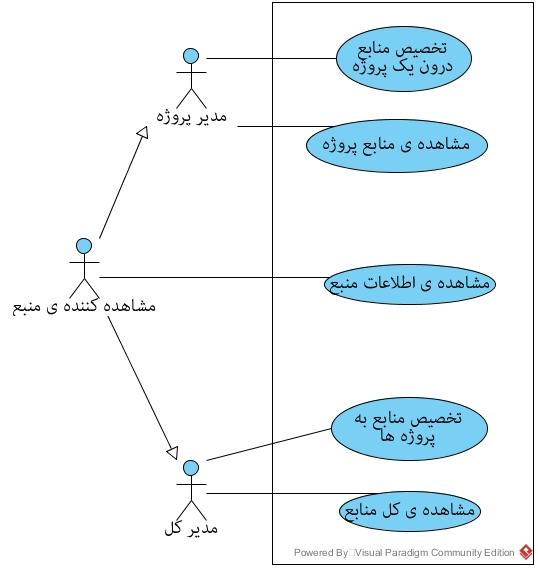
\includegraphics[width=0.7\textwidth]{Diagrams/Resources.jpg}
\end{center}

\newpage

\begin{tabular}{|p{2cm}|p{10cm}|}
\hline
نام
&
مشاهده کل منابع
\\
\hline
شناسه
&
35
\\
\hline
توصیف کوتاه
&
مدیر کل فهرستی از منابع موجود در کل سازمان را مشاهده می کند.
\\
\hline
اکتور اولیه
&
مدیر کل
\\
\hline
اکتور ثانویه
&

\\
\hline
شرایط ابتدایی
&
مدیر در سیستم وارد شده باشد.
\\
\hline
سناریوی اصلی
&
1-مدیر با انتخاب گزینه مشاهده کل منابع، این مورد کاربرد را شروع می کند.
\newline
2-سیستم فهرستی شامل تمامی منابع موجود در سیستم را نمایش می دهد.
\\
\hline
شرایط نهایی
&
نمایش فهرستی منابع موجود
\\
\hline
سناریوی جایگزین
&

\\
\hline
\end{tabular}

\vspace{2cm}

\begin{tabular}{|p{2cm}|p{10cm}|}
\hline
نام
&
مشاهده اطلاعات منبع
\\
\hline
شناسه
&
36
\\
\hline
توصیف کوتاه
&
مشاهده کننده منبع، اطلاعات مربوط به هر منبع و مشغله آن در بازه های زمانی متفاوت را نشان میدهد.
\\
\hline
اکتور اولیه
&
مشاهده کننده ی منبع
\\
\hline
اکتور ثانویه
&

\\
\hline
شرایط ابتدایی
&
مشاهده کننده منبع وارد سیستم شده باشد.
\\
\hline
سناریوی اصلی
&
1-مشاهده کننده منبع با انتخاب گزینه اطلاعات منبع، این مورد کاربرد را شروع می کند.
\newline
2- سیستم تمام پروژه هایی که شامل این منبع بوده اند را برمیگرداند.
\newline
3- پروژه های برگردانده شده به صورت مرتب بر اساس زمان به کاربر نشان داده می شوند.
\\
\hline
شرایط نهایی
&
نمایش مرتب شده پروژه های شامل منبع
\\
\hline
سناریوی جایگزین
&

\\
\hline
\end{tabular}

\vspace{2cm}

\begin{tabular}{|p{2cm}|p{10cm}|}
\hline
نام
&
ویرایش نحوه تخصیص منبع
\\
\hline
شناسه
&
37
\\
\hline
توصیف کوتاه
&
مدیرکل می تواند نحوه تخصیص منبع مورد نظر را ویرایش کند. 
\\
\hline
اکتور اولیه
&
مدیر کل
\\
\hline
اکتور ثانویه
&

\\
\hline
شرایط ابتدایی
&
مدیر کل وارد سیستم شده باشد.
\\
\hline
سناریوی اصلی
&
1-مدیر کل گزینه ویرایش نحوه تخصیص منبع را انتخاب می کند.
\newline
2-مدیر با انتخاب هریک از بازه های زمانی پروژه ای را تغییر داده یا اضافه و یا حذف می کند.
\newline
3- مدیرکل با انتخاب گزینه تایید ویرایش، موافقت خود با ثبت تغییرات را اعلام می کند.
\newline
4- سیستم اطلاعات مربوط به تغییر، حذف یا اضافه شدن منبع به پروژه های مختلف را ذخیره می کند.  
\\
\hline
شرایط نهایی
&
ثبت اطلاعات مربوط به تغییر منابع اختصاص شده به پروژه های مختلف.
\\
\hline
سناریوی جایگزین
&

\\
\hline
\end{tabular}

\vspace{2cm}

\begin{tabular}{|p{2cm}|p{10cm}|}
\hline
نام
&
مشاهده نحوه تخصیص منبع یک پروژه
\\
\hline
شناسه
&
38
\\
\hline
توصیف کوتاه
&
مدیر پروژه فهرستی از منابع موجود در پروژه را مشاهده می کند.
\\
\hline
اکتور اولیه
&
مدیر کل
\\
\hline
اکتور ثانویه
&

\\
\hline
شرایط ابتدایی
&
مدیرپروژه در سیستم وارد شده باشد.
\\
\hline
سناریوی اصلی
&
1-مدیرپروژه با انتخاب گزینه مشاهده منابع، این مورد کاربرد را شروع می کند.
\newline
2-مدیر پروژه پروژه مورد نظر را انتخاب می کند.
\newline
3-مدیر پروژه با انتخاب گزینه تایید، موافقت خود را با پروژه انتخابی نشان می دهد.
\newline
4-سیستم فهرستی شامل منابع مربوط به پروژه انتخاب شده نمایش می دهد.
\\
\hline
شرایط نهایی
&
نمایش فهرستی منابع مربوط به پروژه
\\
\hline
سناریوی جایگزین
&

\\
\hline
\end{tabular}

\vspace{2cm}

\begin{tabular}{|p{2cm}|p{10cm}|}
\hline
نام
&
ویرایش نحوه تخصیص منبع یک پروژه
\\
\hline
شناسه
&
39
\\
\hline
توصیف کوتاه
&
مدیر پروژه می تواند نحوه تخصیص منبع مورد نظر را ویرایش کند. 
\\
\hline
اکتور اولیه
&
مدیر پروژه
\\
\hline
اکتور ثانویه
&

\\
\hline
شرایط ابتدایی
&
مدیر پروژه وارد سیستم شده باشد.
\\
\hline
سناریوی اصلی
&
1-مدیر پروژه گزینه ویرایش نحوه تخصیص منبع را انتخاب می کند.
\newline
2-مدیر با انتخاب هریک از بازه های زمانی ماژولی را تغییر داده یا اضافه و یا حذف می کند.
\newline
3- مدیر پروژه با انتخاب گزینه تایید ویرایش، موافقت خود با ثبت تغییرات را اعلام می کند.
\newline
4- سیستم اطلاعات مربوط به تغییر، حذف یا اضافه شدن منبع به ماژولهای مختلف را ذخیره می کند.  
\\
\hline
شرایط نهایی
&
ثبت اطلاعات مربوط به تغییر منابع اختصاص شده به ماژول‌های مختلف.
\\
\hline
سناریوی جایگزین
&

\\
\hline
\end{tabular}


\newpage
\subsection{زیرسیستم گزارش‌گیری}

\vspace{2cm}
\begin{center}
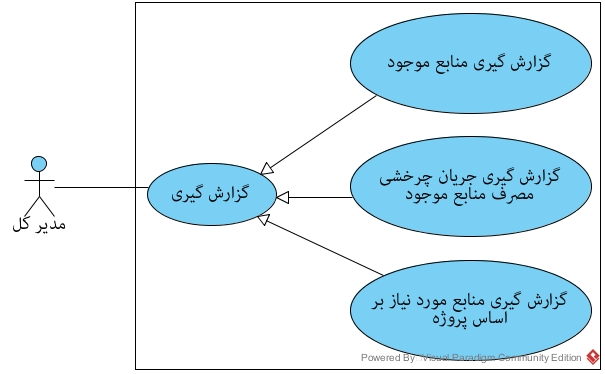
\includegraphics[width=\textwidth]{Diagrams/Reporting.jpg}
\end{center}

\newpage

\begin{tabular}{|p{2cm}|p{10cm}|}
\hline
نام
&
گزارش گیری منابع موجود
\\
\hline
شناسه
&
40
\\
\hline
شناسه پدر
&
43
\\
\hline
توصیف کوتاه
&
گزارشی از اینکه هر منبع به چه میزان و در کدام قسمت موجود است نمایش داده می شود
\\
\hline
اکتور اولیه
&
مدیر کل
\\
\hline
اکتور ثانویه
&

\\
\hline
شرایط ابتدایی
&

\\
\hline
سناریوی اصلی
&
1-مدیر با انتخاب گزارش گیری منابع موجود  این مورد کاربرد را شروع می کند.
\newline
2-مدیر پروژه یا پروژه های مورد نظر خود را مشخص میکند.
\newline
3-با انتخاب گزینه دریافت گزارش ، سیستم منابع موجود در هر قسمت در پروژه/پروژه های مورد نظر را نمایش می دهد. 
\\
\hline
شرایط نهایی
&

\\
\hline
سناریوی جایگزین
&

\\
\hline
\end{tabular}

\vspace{2cm}

\begin{tabular}{|p{2cm}|p{10cm}|}
\hline
نام
&
گزارش گیری جریان چرخشی مصرف منابع موجود
\\
\hline
شناسه
&
41
\\
\hline
شناسه پدر
&
43
\\
\hline
توصیف کوتاه
&
گزارشی حاوی میزان استفاده از منابع تحت عنوان گزارش جریان چرخشی منابع نمایش داده می شود.
\\
\hline
اکتور اولیه
&
مدیر کل
\\
\hline
اکتور ثانویه
&

\\
\hline
شرایط ابتدایی
&

\\
\hline
سناریوی اصلی
&
1-مدیر با انتخاب گزارش گیری جریان چرخشی مصرف منابع موجود این مورد کاربرد را شروع می کند.
\newline
2-مدیر بازه زمانی مورد نظر خود را وارد میکند.
\newline
3-با انتخاب گزینه دریافت گزارش، سیستم میزان استفاده از منابع موجود در هر قسمت در بازه زمانی مورد نظر را نمایش می دهد. 
\\
\hline
شرایط نهایی
&

\\
\hline
سناریوی جایگزین
&

\\
\hline
\end{tabular}

\vspace{2cm}

\begin{tabular}{|p{2cm}|p{10cm}|}
\hline
نام
&
گزارش گیری منابع مورد نیاز براساس پروژه
\\
\hline
شناسه
&
42
\\
\hline
شناسه پدر
&
43
\\
\hline
توصیف کوتاه
&
گزارش حاوی منابع موجود در هر پروژه نمایش داده می شود.
\\
\hline
اکتور اولیه
&
مدیر کل
\\
\hline
اکتور ثانویه
&

\\
\hline
شرایط ابتدایی
&

\\
\hline
سناریوی اصلی
&
1-مدیر با انتخاب گزارش گیری منابع مورد نیاز براساس پروژه این مورد کاربرد را شروع می کند.
\newline
2-مدیر پروژه یا پروژه های مورد نظر خود را مشخص میکند. 
\newline
3-با انتخاب گزینه دریافت گزارش، سیستم  منابع مورد استفاده در پروژه/پروژه های مورد نظر را نمایش می دهد. 

\\
\hline
شرایط نهایی
&

\\
\hline
سناریوی جایگزین
&

\\
\hline
\end{tabular}

\vspace{2cm}

\begin{tabular}{|p{2cm}|p{10cm}|}
\hline
نام
&
گزارش گیری
\\
\hline
شناسه
&
43
\\
\hline
توصیف کوتاه
&
گزارشی از منابع توسط مدیر دریافت می شود.
\\
\hline
اکتور اولیه
&
مدیر کل 
\\
\hline
اکتور ثانویه
&

\\
\hline
شرایط ابتدایی
&
مدیر وارد حساب کاربری خود شده باشد
\\
\hline
سناریوی اصلی
&

\\
\hline
شرایط نهایی
&
گزارش از سیستم گرفته می شود.
\\
\hline
سناریوی جایگزین
&

\\
\hline
\end{tabular}



\newpage
\subsection{زیرسیستم پیش‌بینی}

\vspace{2cm}
\begin{center}
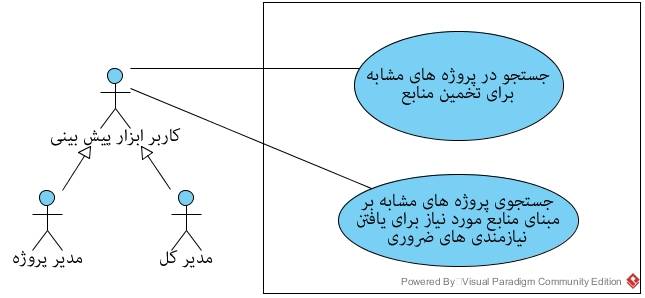
\includegraphics[width=\textwidth]{Diagrams/Anticipating.jpg}
\end{center}


\newpage
\begin{tabular}{|p{2cm}|p{10cm}|}
\hline
نام
&
جستجو در پروژه های مشابه برای تخمین منابع
\\
\hline
شناسه
&
44
\\
\hline
توصیف کوتاه
&
کاربر ابزار پیش‌بینی در میان پروژه‌های موجود بر اساس ویژگی‌های مختلف جستجو می‌کند.
\\
\hline
اکتور اولیه
&
کاربر ابزار پیش‌بینی
\\
\hline
اکتور ثانویه
&

\\
\hline
شرایط ابتدایی
&
کاربر ابزار پیش‌بینی در سیستم وارد شده باشد.
\\
\hline
سناریوی اصلی
&
1- کاربر ابزار پیش‌بینی با انتخاب گزینه‌ی جستجوی پروژه، این مورد کاربرد را شروع می‌کند.
\newline
2- کاربر ابزار پیش‌بینی بازه‌ی سایز و تکنولوژی مورد نظرش را وارد می‌کند.
\newline
3- سیستم فهرستی از پروژه‌ها با ویژگی‌های مورد نظر را نمایش می‌دهد.
\\
\hline
شرایط نهایی
&
فهرستی از پروژه‌ها با ویژگی‌های مورد نظر نمایش داده می‌شود.
\\
\hline
سناریوی جایگزین
&

\\
\hline
\end{tabular}

\vspace{2cm}

\begin{tabular}{|p{2cm}|p{10cm}|}
\hline
نام
&
جستجوی پروژه های مشابه بر مبنای منابع مورد نیاز برای یافتن نیازمندی های ضروری
\\
\hline
شناسه
&
45
\\
\hline
توصیف کوتاه
&
کاربر ابزار پیش‌بینی در میان پروژه‌های موجود بر اساس منابع مورد نیاز، جستجو می‌کند.
\\
\hline
اکتور اولیه
&
کاربر ابزار پیش‌بینی
\\
\hline
اکتور ثانویه
&

\\
\hline
شرایط ابتدایی
&
کاربر ابزار پیش‌بینی در سیستم وارد شده باشد.
\\
\hline
سناریوی اصلی
&
1- کاربر ابزار پیش‌بینی با انتخاب گزینه‌ی جستجو بر اساس منابع، این مورد کاربرد را شروع می‌کند.
\newline
2- کاربر ابزار پیش‌بینی منابع مورد نیاز را وارد می‌کند.
\newline
3- سیستم فهرستی از پروژه‌ها با منابع مشابه و نیازمندی‌های ضروری این پروژه‌ها را نمایش می‌دهد.
\\
\hline
شرایط نهایی
&
فهرستی از پروژه‌ها با منابع مشابه و نیازمندی‌های ضروری آن‌ها نشان داده می‌شود.
\\
\hline
سناریوی جایگزین
&

\\
\hline
\end{tabular}